\documentclass[twoside]{book}

% Packages required by doxygen
\usepackage{fixltx2e}
\usepackage{calc}
\usepackage{doxygen}
\usepackage[export]{adjustbox} % also loads graphicx
\usepackage{graphicx}
\usepackage[utf8]{inputenc}
\usepackage{makeidx}
\usepackage{multicol}
\usepackage{multirow}
\PassOptionsToPackage{warn}{textcomp}
\usepackage{textcomp}
\usepackage[nointegrals]{wasysym}
\usepackage[table]{xcolor}

% Font selection
\usepackage[T1]{fontenc}
\usepackage[scaled=.90]{helvet}
\usepackage{courier}
\usepackage{amssymb}
\usepackage{sectsty}
\renewcommand{\familydefault}{\sfdefault}
\allsectionsfont{%
  \fontseries{bc}\selectfont%
  \color{darkgray}%
}
\renewcommand{\DoxyLabelFont}{%
  \fontseries{bc}\selectfont%
  \color{darkgray}%
}
\newcommand{\+}{\discretionary{\mbox{\scriptsize$\hookleftarrow$}}{}{}}

% Page & text layout
\usepackage{geometry}
\geometry{%
  a4paper,%
  top=2.5cm,%
  bottom=2.5cm,%
  left=2.5cm,%
  right=2.5cm%
}
\tolerance=750
\hfuzz=15pt
\hbadness=750
\setlength{\emergencystretch}{15pt}
\setlength{\parindent}{0cm}
\setlength{\parskip}{3ex plus 2ex minus 2ex}
\makeatletter
\renewcommand{\paragraph}{%
  \@startsection{paragraph}{4}{0ex}{-1.0ex}{1.0ex}{%
    \normalfont\normalsize\bfseries\SS@parafont%
  }%
}
\renewcommand{\subparagraph}{%
  \@startsection{subparagraph}{5}{0ex}{-1.0ex}{1.0ex}{%
    \normalfont\normalsize\bfseries\SS@subparafont%
  }%
}
\makeatother

% Headers & footers
\usepackage{fancyhdr}
\pagestyle{fancyplain}
\fancyhead[LE]{\fancyplain{}{\bfseries\thepage}}
\fancyhead[CE]{\fancyplain{}{}}
\fancyhead[RE]{\fancyplain{}{\bfseries\leftmark}}
\fancyhead[LO]{\fancyplain{}{\bfseries\rightmark}}
\fancyhead[CO]{\fancyplain{}{}}
\fancyhead[RO]{\fancyplain{}{\bfseries\thepage}}
\fancyfoot[LE]{\fancyplain{}{}}
\fancyfoot[CE]{\fancyplain{}{}}
\fancyfoot[RE]{\fancyplain{}{\bfseries\scriptsize Generated by Doxygen }}
\fancyfoot[LO]{\fancyplain{}{\bfseries\scriptsize Generated by Doxygen }}
\fancyfoot[CO]{\fancyplain{}{}}
\fancyfoot[RO]{\fancyplain{}{}}
\renewcommand{\footrulewidth}{0.4pt}
\renewcommand{\chaptermark}[1]{%
  \markboth{#1}{}%
}
\renewcommand{\sectionmark}[1]{%
  \markright{\thesection\ #1}%
}

% Indices & bibliography
\usepackage{natbib}
\usepackage[titles]{tocloft}
\setcounter{tocdepth}{3}
\setcounter{secnumdepth}{5}
\makeindex

% Hyperlinks (required, but should be loaded last)
\usepackage{ifpdf}
\ifpdf
  \usepackage[pdftex,pagebackref=true]{hyperref}
\else
  \usepackage[ps2pdf,pagebackref=true]{hyperref}
\fi
\hypersetup{%
  colorlinks=true,%
  linkcolor=blue,%
  citecolor=blue,%
  unicode%
}

% Custom commands
\newcommand{\clearemptydoublepage}{%
  \newpage{\pagestyle{empty}\cleardoublepage}%
}

\usepackage{caption}
\captionsetup{labelsep=space,justification=centering,font={bf},singlelinecheck=off,skip=4pt,position=top}

%===== C O N T E N T S =====

\begin{document}

% Titlepage & ToC
\hypersetup{pageanchor=false,
             bookmarksnumbered=true,
             pdfencoding=unicode
            }
\pagenumbering{roman}
\begin{titlepage}
\vspace*{7cm}
\begin{center}%
{\Large cascadable\+\_\+counter }\\
\vspace*{1cm}
{\large Generated by Doxygen 1.8.11}\\
\end{center}
\end{titlepage}
\clearemptydoublepage
\tableofcontents
\clearemptydoublepage
\pagenumbering{arabic}
\hypersetup{pageanchor=true}

%--- Begin generated contents ---
\chapter{Design Unit Index}
\section{Design Unit Hierarchy}
This inheritance list is sorted roughly, but not completely, alphabetically\+:\begin{DoxyCompactList}
\item \contentsline{section}{tb\+\_\+\+Flip\+\_\+flop\+\_\+\+R\+\_\+W}{\pageref{classtb___flip__flop___r___w}}{}
\begin{DoxyCompactList}
\item \contentsline{section}{Flip\+\_\+flop\+\_\+\+R\+\_\+W}{\pageref{class_flip__flop___r___w}}{}
\end{DoxyCompactList}
\item \contentsline{section}{tb\+\_\+\+Flip\+\_\+flop\+\_\+\+R\+C\+\_\+S}{\pageref{classtb___flip__flop___r_c___s}}{}
\begin{DoxyCompactList}
\item \contentsline{section}{Flip\+\_\+flop\+\_\+\+R\+C\+\_\+S}{\pageref{class_flip__flop___r_c___s}}{}
\end{DoxyCompactList}
\end{DoxyCompactList}

\chapter{Design Unit Index}
\section{Design Unit List}
Here is a list of all design unit members with links to the Entities they belong to\+:\begin{DoxyCompactList}
\item\contentsline{section}{architecture \hyperlink{classtb__cascadable__counter_1_1_behavioral}{Behavioral} \\*Architecture definition of the \hyperlink{classtb__cascadable__counter}{tb\+\_\+cascadable\+\_\+counter} }{\pageref{classtb__cascadable__counter_1_1_behavioral}}{}
\item\contentsline{section}{entity \hyperlink{classcascadable__counter}{cascadable\+\_\+counter} }{\pageref{classcascadable__counter}}{}
\item\contentsline{section}{architecture \hyperlink{classcascadable__counter_1_1fsm}{fsm} \\*Architecture definition of the \hyperlink{classcascadable__counter}{cascadable\+\_\+counter} }{\pageref{classcascadable__counter_1_1fsm}}{}
\item\contentsline{section}{entity \hyperlink{classtb__cascadable__counter}{tb\+\_\+cascadable\+\_\+counter} }{\pageref{classtb__cascadable__counter}}{}
\end{DoxyCompactList}

\chapter{File Index}
\section{File List}
Here is a list of all documented files with brief descriptions\+:\begin{DoxyCompactList}
\item\contentsline{section}{C\+:/\+Users/\+Public/\+Documents/\+Github/\+V\+H\+D\+L/\+Flip\+\_\+flop/\hyperlink{_flip__flop___r___w_8vhd}{Flip\+\_\+flop\+\_\+\+R\+\_\+\+W.\+vhd} \\*\hyperlink{class_flip__flop___r___w}{Flip\+\_\+flop\+\_\+\+R\+\_\+W} \+: This entity with synchronization reset is uesd to perform a special port. It could be read by microcontroller and writen by I2C. That means if I2C set \textquotesingle{}i2c\+\_\+write\textquotesingle{} on one, it would put the data of \textquotesingle{}i2c\+\_\+data\+\_\+in\textquotesingle{} into the output \textquotesingle{}uc\+\_\+read\textquotesingle{}. It could be one or zero.\+It just likes its write fonction. Then we can use its output as the input of microcontroller. It likes read by microcontroller }{\pageref{_flip__flop___r___w_8vhd}}{}
\item\contentsline{section}{C\+:/\+Users/\+Public/\+Documents/\+Github/\+V\+H\+D\+L/\+Flip\+\_\+flop/\hyperlink{_flip__flop___r_c___s_8vhd}{Flip\+\_\+flop\+\_\+\+R\+C\+\_\+\+S.\+vhd} \\*\hyperlink{class_flip__flop___r_c___s}{Flip\+\_\+flop\+\_\+\+R\+C\+\_\+S} \+: This entity with synchronization reset is uesd to perform a special port. It could be read or cleared by microcontroller and writen by I2C. That means if microcontroller set \textquotesingle{}uc\+\_\+clear\textquotesingle{} on one, it would set the output on zero. If I2C set \textquotesingle{}i2c\+\_\+set\textquotesingle{} on one, it would set the output on one. It just likes its set fonction. Then we can use its output as the input of microcontroller. It likes read by microcontroller }{\pageref{_flip__flop___r_c___s_8vhd}}{}
\item\contentsline{section}{C\+:/\+Users/\+Public/\+Documents/\+Github/\+V\+H\+D\+L/\+Flip\+\_\+flop/\hyperlink{tb___flip__flop___r___w_8vhd}{tb\+\_\+\+Flip\+\_\+flop\+\_\+\+R\+\_\+\+W.\+vhd} \\*Tb\+\_\+\+Flip\+\_\+flop\+\_\+\+R\+\_\+W \+:testbench for the entity flip\+\_\+flop\+\_\+r\+\_\+w }{\pageref{tb___flip__flop___r___w_8vhd}}{}
\item\contentsline{section}{C\+:/\+Users/\+Public/\+Documents/\+Github/\+V\+H\+D\+L/\+Flip\+\_\+flop/\hyperlink{tb___flip__flop___r_c___s_8vhd}{tb\+\_\+\+Flip\+\_\+flop\+\_\+\+R\+C\+\_\+\+S.\+vhd} \\*Tb\+\_\+\+Flip\+\_\+flop\+\_\+\+R\+C\+\_\+S \+:testbench for the entity flip\+\_\+flop\+\_\+rc\+\_\+s }{\pageref{tb___flip__flop___r_c___s_8vhd}}{}
\end{DoxyCompactList}

\chapter{Class Documentation}
\hypertarget{classtb__cascadable__counter_1_1_behavioral}{}\section{Behavioral Architecture Reference}
\label{classtb__cascadable__counter_1_1_behavioral}\index{Behavioral@{Behavioral}}


Architecture definition of the \hyperlink{classtb__cascadable__counter}{tb\+\_\+cascadable\+\_\+counter}.  


\subsection*{Processes}
 \begin{DoxyCompactItemize}
\item 
\hyperlink{classtb__cascadable__counter_1_1_behavioral_a99f3164d142507cc4972fec85ccfe73a}{clk\+\_\+signal}{\bfseries  (  )}\hypertarget{classtb__cascadable__counter_1_1_behavioral_a99f3164d142507cc4972fec85ccfe73a}{}\label{classtb__cascadable__counter_1_1_behavioral_a99f3164d142507cc4972fec85ccfe73a}

\begin{DoxyCompactList}\small\item\em process of generating a clock signal \end{DoxyCompactList}\end{DoxyCompactItemize}
\subsection*{Components}
 \begin{DoxyCompactItemize}
\item 
\hyperlink{classtb__cascadable__counter_1_1_behavioral_a43b32943cff2ea9c75d864730f7a4f8e}{cascadable\+\_\+counter}  {\bfseries }  \hypertarget{classtb__cascadable__counter_1_1_behavioral_a43b32943cff2ea9c75d864730f7a4f8e}{}\label{classtb__cascadable__counter_1_1_behavioral_a43b32943cff2ea9c75d864730f7a4f8e}

\begin{DoxyCompactList}\small\item\em use a entity as a component \end{DoxyCompactList}\end{DoxyCompactItemize}
\subsection*{Signals}
 \begin{DoxyCompactItemize}
\item 
\hyperlink{classtb__cascadable__counter_1_1_behavioral_aed2cb56a5e81f2bcf0aa5c059163934b}{clk} {\bfseries \textcolor{vhdlchar}{S\+T\+D\+\_\+\+L\+O\+G\+IC}\textcolor{vhdlchar}{ }} \hypertarget{classtb__cascadable__counter_1_1_behavioral_aed2cb56a5e81f2bcf0aa5c059163934b}{}\label{classtb__cascadable__counter_1_1_behavioral_aed2cb56a5e81f2bcf0aa5c059163934b}

\begin{DoxyCompactList}\small\item\em use signals internals simulate these ports of component \end{DoxyCompactList}\item 
\hyperlink{classtb__cascadable__counter_1_1_behavioral_a7e333d8b89f48acd3c4ac58948c1afb8}{clk\+\_\+ena} {\bfseries \textcolor{vhdlchar}{S\+T\+D\+\_\+\+L\+O\+G\+IC}\textcolor{vhdlchar}{ }} \hypertarget{classtb__cascadable__counter_1_1_behavioral_a7e333d8b89f48acd3c4ac58948c1afb8}{}\label{classtb__cascadable__counter_1_1_behavioral_a7e333d8b89f48acd3c4ac58948c1afb8}

\item 
\hyperlink{classtb__cascadable__counter_1_1_behavioral_a5d1d334866b850ea4519655e35c948b9}{sync\+\_\+rst} {\bfseries \textcolor{vhdlchar}{S\+T\+D\+\_\+\+L\+O\+G\+IC}\textcolor{vhdlchar}{ }} \hypertarget{classtb__cascadable__counter_1_1_behavioral_a5d1d334866b850ea4519655e35c948b9}{}\label{classtb__cascadable__counter_1_1_behavioral_a5d1d334866b850ea4519655e35c948b9}

\item 
\hyperlink{classtb__cascadable__counter_1_1_behavioral_a94257cdd5b38f9fec342449b8c19eecf}{cascade\+\_\+in} {\bfseries \textcolor{vhdlchar}{S\+T\+D\+\_\+\+L\+O\+G\+IC}\textcolor{vhdlchar}{ }} \hypertarget{classtb__cascadable__counter_1_1_behavioral_a94257cdd5b38f9fec342449b8c19eecf}{}\label{classtb__cascadable__counter_1_1_behavioral_a94257cdd5b38f9fec342449b8c19eecf}

\item 
\hyperlink{classtb__cascadable__counter_1_1_behavioral_aa72821ce86518fa49cef6a2dd942c0ec}{count} {\bfseries \textcolor{vhdlchar}{integer}\textcolor{vhdlchar}{ }} \hypertarget{classtb__cascadable__counter_1_1_behavioral_aa72821ce86518fa49cef6a2dd942c0ec}{}\label{classtb__cascadable__counter_1_1_behavioral_aa72821ce86518fa49cef6a2dd942c0ec}

\item 
\hyperlink{classtb__cascadable__counter_1_1_behavioral_afaaef471ea85496d3f84ba933805bd9b}{cascade\+\_\+out} {\bfseries \textcolor{vhdlchar}{S\+T\+D\+\_\+\+L\+O\+G\+IC}\textcolor{vhdlchar}{ }} \hypertarget{classtb__cascadable__counter_1_1_behavioral_afaaef471ea85496d3f84ba933805bd9b}{}\label{classtb__cascadable__counter_1_1_behavioral_afaaef471ea85496d3f84ba933805bd9b}

\end{DoxyCompactItemize}
\subsection*{Instantiations}
 \begin{DoxyCompactItemize}
\item 
\hyperlink{classtb__cascadable__counter_1_1_behavioral_a6ab2b7ae21cf93d9867b638ede4dbb64}{gen\+\_\+ena}  {\bfseries cascadable\+\_\+counter}   \hypertarget{classtb__cascadable__counter_1_1_behavioral_a6ab2b7ae21cf93d9867b638ede4dbb64}{}\label{classtb__cascadable__counter_1_1_behavioral_a6ab2b7ae21cf93d9867b638ede4dbb64}

\begin{DoxyCompactList}\small\item\em an instance of component \end{DoxyCompactList}\end{DoxyCompactItemize}


\subsection{Detailed Description}
Architecture definition of the \hyperlink{classtb__cascadable__counter}{tb\+\_\+cascadable\+\_\+counter}. 

More details about this \hyperlink{classtb__cascadable__counter}{tb\+\_\+cascadable\+\_\+counter} element. 

The documentation for this class was generated from the following file\+:\begin{DoxyCompactItemize}
\item 
C\+:/\+Users/\+Public/\+Documents/\+Github/\+V\+H\+D\+L/cascadable\+\_\+counter/\hyperlink{tb__cascadable__counter_8vhd}{tb\+\_\+cascadable\+\_\+counter.\+vhd}\end{DoxyCompactItemize}

\hypertarget{classcascadable__counter}{}\section{cascadable\+\_\+counter Entity Reference}
\label{classcascadable__counter}\index{cascadable\+\_\+counter@{cascadable\+\_\+counter}}
Inheritance diagram for cascadable\+\_\+counter\+:\begin{figure}[H]
\begin{center}
\leavevmode
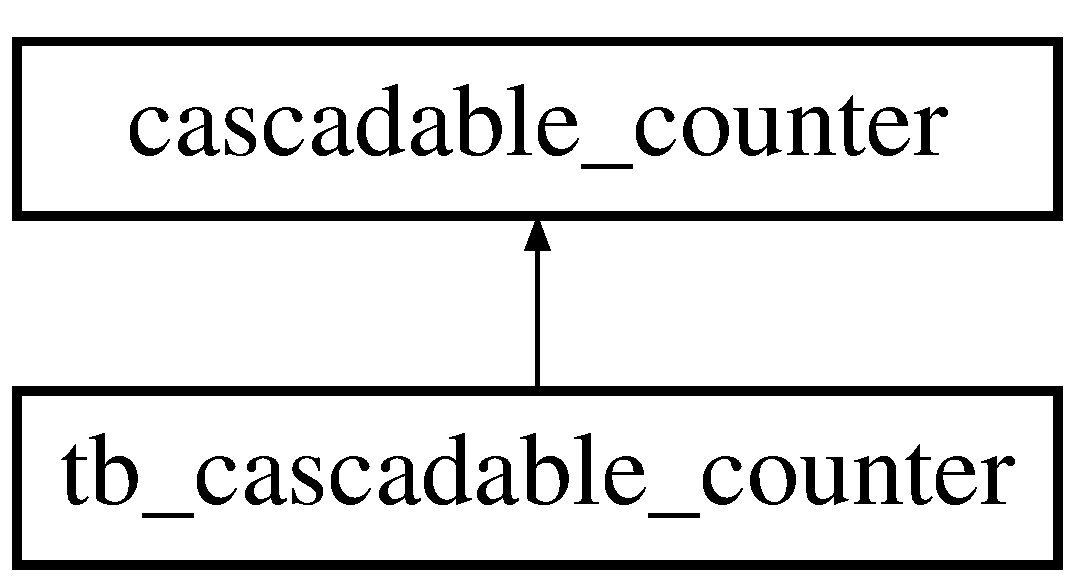
\includegraphics[height=2.000000cm]{classcascadable__counter}
\end{center}
\end{figure}
\subsection*{Entities}
\begin{DoxyCompactItemize}
\item 
\hyperlink{classcascadable__counter_1_1fsm}{fsm} architecture
\begin{DoxyCompactList}\small\item\em Architecture definition of the \hyperlink{classcascadable__counter}{cascadable\+\_\+counter}. \end{DoxyCompactList}\end{DoxyCompactItemize}
\subsection*{Libraries}
 \begin{DoxyCompactItemize}
\item 
\hyperlink{classcascadable__counter_ae4f03c286607f3181e16b9aa12d0c6d4}{I\+E\+EE} \hypertarget{classcascadable__counter_ae4f03c286607f3181e16b9aa12d0c6d4}{}\label{classcascadable__counter_ae4f03c286607f3181e16b9aa12d0c6d4}

\begin{DoxyCompactList}\small\item\em Use standard library. \end{DoxyCompactList}\end{DoxyCompactItemize}
\subsection*{Use Clauses}
 \begin{DoxyCompactItemize}
\item 
\hyperlink{classcascadable__counter_aa4b2b25246a821511120e3149b003563}{S\+T\+D\+\_\+\+L\+O\+G\+I\+C\+\_\+1164}   \hypertarget{classcascadable__counter_aa4b2b25246a821511120e3149b003563}{}\label{classcascadable__counter_aa4b2b25246a821511120e3149b003563}

\begin{DoxyCompactList}\small\item\em Use logic elements. \end{DoxyCompactList}\end{DoxyCompactItemize}
\subsection*{Generics}
 \begin{DoxyCompactItemize}
\item 
\hyperlink{classcascadable__counter_af71dfc83a4840a03979233942440efbb}{divisor} {\bfseries {\bfseries \textcolor{vhdlchar}{positive}\textcolor{vhdlchar}{ }\textcolor{vhdlchar}{ }\textcolor{vhdlchar}{\+:}\textcolor{vhdlchar}{=}\textcolor{vhdlchar}{ }\textcolor{vhdlchar}{ } \textcolor{vhdldigit}{2} \textcolor{vhdlchar}{ }}}\hypertarget{classcascadable__counter_af71dfc83a4840a03979233942440efbb}{}\label{classcascadable__counter_af71dfc83a4840a03979233942440efbb}

\end{DoxyCompactItemize}
\subsection*{Ports}
 \begin{DoxyCompactItemize}
\item 
\hyperlink{classcascadable__counter_a6231b307b7958b6060563aa2a93d345a}{clk}  {\bfseries {\bfseries \textcolor{vhdlchar}{in}\textcolor{vhdlchar}{ }}} {\bfseries \textcolor{vhdlchar}{S\+T\+D\+\_\+\+L\+O\+G\+IC}\textcolor{vhdlchar}{ }} \hypertarget{classcascadable__counter_a6231b307b7958b6060563aa2a93d345a}{}\label{classcascadable__counter_a6231b307b7958b6060563aa2a93d345a}

\begin{DoxyCompactList}\small\item\em clock input \end{DoxyCompactList}\item 
\hyperlink{classcascadable__counter_a3313e71ab116de6fc03014f85009a19d}{clk\+\_\+ena}  {\bfseries {\bfseries \textcolor{vhdlchar}{in}\textcolor{vhdlchar}{ }}} {\bfseries \textcolor{vhdlchar}{S\+T\+D\+\_\+\+L\+O\+G\+IC}\textcolor{vhdlchar}{ }} \hypertarget{classcascadable__counter_a3313e71ab116de6fc03014f85009a19d}{}\label{classcascadable__counter_a3313e71ab116de6fc03014f85009a19d}

\begin{DoxyCompactList}\small\item\em clock\+\_\+enable input \end{DoxyCompactList}\item 
\hyperlink{classcascadable__counter_a3495b88db081463071853b171449fc35}{sync\+\_\+rst}  {\bfseries {\bfseries \textcolor{vhdlchar}{in}\textcolor{vhdlchar}{ }}} {\bfseries \textcolor{vhdlchar}{S\+T\+D\+\_\+\+L\+O\+G\+IC}\textcolor{vhdlchar}{ }} \hypertarget{classcascadable__counter_a3495b88db081463071853b171449fc35}{}\label{classcascadable__counter_a3495b88db081463071853b171449fc35}

\begin{DoxyCompactList}\small\item\em synchronization reset input \end{DoxyCompactList}\item 
\hyperlink{classcascadable__counter_a4a6788b2a9d396f8a12b03ff15c3899d}{cascade\+\_\+in}  {\bfseries {\bfseries \textcolor{vhdlchar}{in}\textcolor{vhdlchar}{ }}} {\bfseries \textcolor{vhdlchar}{S\+T\+D\+\_\+\+L\+O\+G\+IC}\textcolor{vhdlchar}{ }} \hypertarget{classcascadable__counter_a4a6788b2a9d396f8a12b03ff15c3899d}{}\label{classcascadable__counter_a4a6788b2a9d396f8a12b03ff15c3899d}

\begin{DoxyCompactList}\small\item\em cascade\+\_\+in input \end{DoxyCompactList}\item 
\hyperlink{classcascadable__counter_aaca90a4bb78d0c63502de161d6f2197c}{count}  {\bfseries {\bfseries \textcolor{vhdlchar}{out}\textcolor{vhdlchar}{ }}} {\bfseries \textcolor{vhdlchar}{integer}\textcolor{vhdlchar}{ }\textcolor{vhdlchar}{ }\textcolor{vhdlchar}{ }\textcolor{vhdlchar}{range}\textcolor{vhdlchar}{ }\textcolor{vhdlchar}{ } \textcolor{vhdldigit}{0} \textcolor{vhdlchar}{ }\textcolor{vhdlchar}{to}\textcolor{vhdlchar}{ }\textcolor{vhdlchar}{(}\textcolor{vhdlchar}{ }\textcolor{vhdlchar}{ }\textcolor{vhdlchar}{ }\textcolor{vhdlchar}{ }\textcolor{vhdlchar}{divisor}\textcolor{vhdlchar}{-\/}\textcolor{vhdlchar}{ } \textcolor{vhdldigit}{1} \textcolor{vhdlchar}{ }\textcolor{vhdlchar}{)}\textcolor{vhdlchar}{ }} \hypertarget{classcascadable__counter_aaca90a4bb78d0c63502de161d6f2197c}{}\label{classcascadable__counter_aaca90a4bb78d0c63502de161d6f2197c}

\begin{DoxyCompactList}\small\item\em count by variable \end{DoxyCompactList}\item 
\hyperlink{classcascadable__counter_aebe3fcbeecb083647db0f3cfb205d03d}{cascade\+\_\+out}  {\bfseries {\bfseries \textcolor{vhdlchar}{out}\textcolor{vhdlchar}{ }}} {\bfseries \textcolor{vhdlchar}{S\+T\+D\+\_\+\+L\+O\+G\+IC}\textcolor{vhdlchar}{ }} \hypertarget{classcascadable__counter_aebe3fcbeecb083647db0f3cfb205d03d}{}\label{classcascadable__counter_aebe3fcbeecb083647db0f3cfb205d03d}

\begin{DoxyCompactList}\small\item\em maximum count then works \end{DoxyCompactList}\end{DoxyCompactItemize}


\subsection{Detailed Description}
\hyperlink{classcascadable__counter}{cascadable\+\_\+counter} entity brief description Detailed description of this \hyperlink{classcascadable__counter}{cascadable\+\_\+counter} design element. 

The documentation for this class was generated from the following file\+:\begin{DoxyCompactItemize}
\item 
C\+:/\+Users/\+Public/\+Documents/\+Github/\+V\+H\+D\+L/cascadable\+\_\+counter/\hyperlink{cascadable__counter_8vhd}{cascadable\+\_\+counter.\+vhd}\end{DoxyCompactItemize}

\hypertarget{classcascadable__counter_1_1fsm}{}\section{fsm Architecture Reference}
\label{classcascadable__counter_1_1fsm}\index{fsm@{fsm}}


Architecture definition of the \hyperlink{classcascadable__counter}{cascadable\+\_\+counter}.  


\subsection*{Processes}
 \begin{DoxyCompactItemize}
\item 
\hyperlink{classcascadable__counter_1_1fsm_aca869937c40a3cb0b3e8467b28f4c42b}{transitions\+\_\+and\+\_\+storage}{\bfseries  ( {\bfseries {\bfseries \hyperlink{classcascadable__counter_a6231b307b7958b6060563aa2a93d345a}{clk}} \textcolor{vhdlchar}{ }} )}
\begin{DoxyCompactList}\small\item\em Process transitions\+\_\+and\+\_\+storage of the Architecture. \end{DoxyCompactList}\item 
\hyperlink{classcascadable__counter_1_1fsm_a1d677b6bb6166ce57abc767d771832b1}{stateaction}{\bfseries  ( {\bfseries \textcolor{vhdlchar}{count\+\_\+state}\textcolor{vhdlchar}{ }} )}\hypertarget{classcascadable__counter_1_1fsm_a1d677b6bb6166ce57abc767d771832b1}{}\label{classcascadable__counter_1_1fsm_a1d677b6bb6166ce57abc767d771832b1}

\begin{DoxyCompactList}\small\item\em if the sync\+\_\+rst equal to \textquotesingle{}0\textquotesingle{}, after the rising\+\_\+edge, we\textquotesingle{}ll reset the count\+\_\+state \end{DoxyCompactList}\end{DoxyCompactItemize}
\subsection*{Signals}
 \begin{DoxyCompactItemize}
\item 
\hyperlink{classcascadable__counter_1_1fsm_a17cbd5b34591bc118d423ba7b7a733aa}{count\+\_\+state} {\bfseries \textcolor{vhdlchar}{integer}\textcolor{vhdlchar}{ }\textcolor{vhdlchar}{ }\textcolor{vhdlchar}{ }\textcolor{vhdlchar}{range}\textcolor{vhdlchar}{ }\textcolor{vhdlchar}{ } \textcolor{vhdldigit}{0} \textcolor{vhdlchar}{ }\textcolor{vhdlchar}{to}\textcolor{vhdlchar}{ }\textcolor{vhdlchar}{(}\textcolor{vhdlchar}{ }\textcolor{vhdlchar}{ }\textcolor{vhdlchar}{ }\textcolor{vhdlchar}{ }\textcolor{vhdlchar}{divisor}\textcolor{vhdlchar}{-\/}\textcolor{vhdlchar}{ } \textcolor{vhdldigit}{1} \textcolor{vhdlchar}{ }\textcolor{vhdlchar}{)}\textcolor{vhdlchar}{ }} \hypertarget{classcascadable__counter_1_1fsm_a17cbd5b34591bc118d423ba7b7a733aa}{}\label{classcascadable__counter_1_1fsm_a17cbd5b34591bc118d423ba7b7a733aa}

\end{DoxyCompactItemize}


\subsection{Detailed Description}
Architecture definition of the \hyperlink{classcascadable__counter}{cascadable\+\_\+counter}. 

More details about this \hyperlink{classcascadable__counter}{cascadable\+\_\+counter} element. 

\subsection{Member Function Documentation}
\index{cascadable\+\_\+counter\+::fsm@{cascadable\+\_\+counter\+::fsm}!transitions\+\_\+and\+\_\+storage@{transitions\+\_\+and\+\_\+storage}}
\index{transitions\+\_\+and\+\_\+storage@{transitions\+\_\+and\+\_\+storage}!cascadable\+\_\+counter\+::fsm@{cascadable\+\_\+counter\+::fsm}}
\subsubsection[{\texorpdfstring{transitions\+\_\+and\+\_\+storageclk}{transitions_and_storageclk}}]{\setlength{\rightskip}{0pt plus 5cm} {\bfseries \textcolor{vhdlchar}{ }} transitions\+\_\+and\+\_\+storage(
\begin{DoxyParamCaption}
\item[{}]{{\bfseries {\bfseries {\bf clk}} \textcolor{vhdlchar}{ }} {\em }}
\end{DoxyParamCaption}
)\hspace{0.3cm}{\ttfamily [Process]}}\hypertarget{classcascadable__counter_1_1fsm_aca869937c40a3cb0b3e8467b28f4c42b}{}\label{classcascadable__counter_1_1fsm_aca869937c40a3cb0b3e8467b28f4c42b}


Process transitions\+\_\+and\+\_\+storage of the Architecture. 

More details about this transitions\+\_\+and\+\_\+storage element. 

The documentation for this class was generated from the following file\+:\begin{DoxyCompactItemize}
\item 
C\+:/\+Users/\+Public/\+Documents/\+Github/\+V\+H\+D\+L/cascadable\+\_\+counter/\hyperlink{cascadable__counter_8vhd}{cascadable\+\_\+counter.\+vhd}\end{DoxyCompactItemize}

\hypertarget{classtb__cascadable__counter}{}\section{tb\+\_\+cascadable\+\_\+counter Entity Reference}
\label{classtb__cascadable__counter}\index{tb\+\_\+cascadable\+\_\+counter@{tb\+\_\+cascadable\+\_\+counter}}
Inheritance diagram for tb\+\_\+cascadable\+\_\+counter\+:\begin{figure}[H]
\begin{center}
\leavevmode
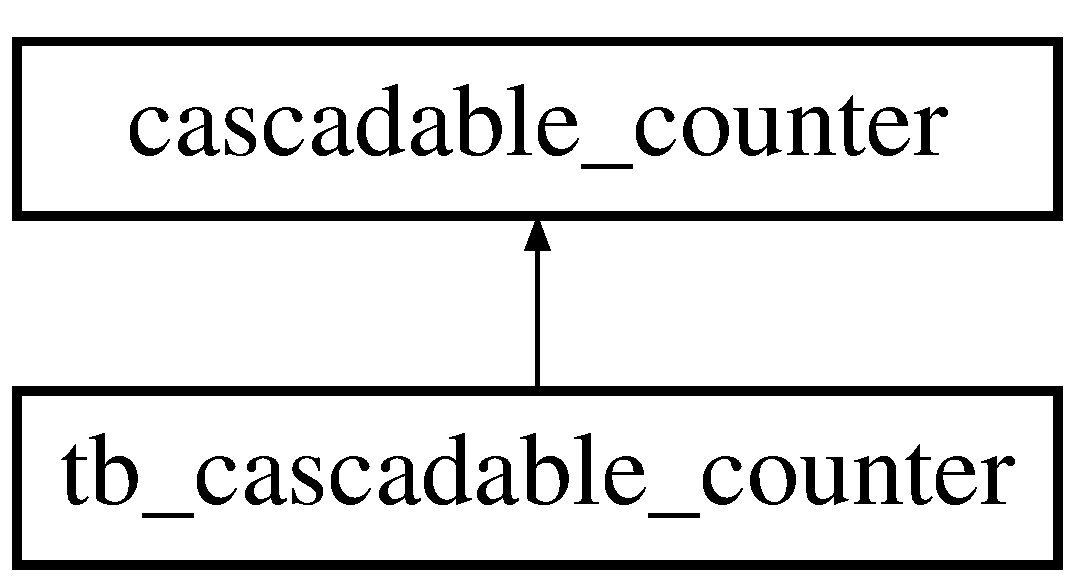
\includegraphics[height=2.000000cm]{classtb__cascadable__counter}
\end{center}
\end{figure}
\subsection*{Entities}
\begin{DoxyCompactItemize}
\item 
\hyperlink{classtb__cascadable__counter_1_1_behavioral}{Behavioral} architecture
\begin{DoxyCompactList}\small\item\em Architecture definition of the \hyperlink{classtb__cascadable__counter}{tb\+\_\+cascadable\+\_\+counter}. \end{DoxyCompactList}\end{DoxyCompactItemize}
\subsection*{Libraries}
 \begin{DoxyCompactItemize}
\item 
\hyperlink{classtb__cascadable__counter_ae4f03c286607f3181e16b9aa12d0c6d4}{I\+E\+EE} \hypertarget{classtb__cascadable__counter_ae4f03c286607f3181e16b9aa12d0c6d4}{}\label{classtb__cascadable__counter_ae4f03c286607f3181e16b9aa12d0c6d4}

\begin{DoxyCompactList}\small\item\em Use standard library. \end{DoxyCompactList}\end{DoxyCompactItemize}
\subsection*{Use Clauses}
 \begin{DoxyCompactItemize}
\item 
\hyperlink{classtb__cascadable__counter_aa4b2b25246a821511120e3149b003563}{S\+T\+D\+\_\+\+L\+O\+G\+I\+C\+\_\+1164}   \hypertarget{classtb__cascadable__counter_aa4b2b25246a821511120e3149b003563}{}\label{classtb__cascadable__counter_aa4b2b25246a821511120e3149b003563}

\begin{DoxyCompactList}\small\item\em Use logic elements. \end{DoxyCompactList}\end{DoxyCompactItemize}


The documentation for this class was generated from the following file\+:\begin{DoxyCompactItemize}
\item 
C\+:/\+Users/\+Public/\+Documents/\+Github/\+V\+H\+D\+L/cascadable\+\_\+counter/\hyperlink{tb__cascadable__counter_8vhd}{tb\+\_\+cascadable\+\_\+counter.\+vhd}\end{DoxyCompactItemize}

\chapter{File Documentation}
\hypertarget{cascadable__counter_8vhd}{}\section{C\+:/\+Users/\+Public/\+Documents/\+Github/\+V\+H\+D\+L/cascadable\+\_\+counter/cascadable\+\_\+counter.vhd File Reference}
\label{cascadable__counter_8vhd}\index{C\+:/\+Users/\+Public/\+Documents/\+Github/\+V\+H\+D\+L/cascadable\+\_\+counter/cascadable\+\_\+counter.\+vhd@{C\+:/\+Users/\+Public/\+Documents/\+Github/\+V\+H\+D\+L/cascadable\+\_\+counter/cascadable\+\_\+counter.\+vhd}}


\hyperlink{classcascadable__counter}{cascadable\+\_\+counter} \+: This entity with synchronization reset is used to count a loop number from zero to maximum value. By the way, we can change the maximum value by change the value on generic. When the number counted arrive to the maximum value,the output \textquotesingle{}count\textquotesingle{} need to be set on zero. At the same time, output \textquotesingle{}cascade\+\_\+out\textquotesingle{} would be set on one for one period. When the \textquotesingle{}count\textquotesingle{} keep on counting, \textquotesingle{}cascade\+\_\+out\textquotesingle{} would be set on zero.  


\subsection*{Entities}
\begin{DoxyCompactItemize}
\item 
\hyperlink{classcascadable__counter}{cascadable\+\_\+counter} entity
\item 
\hyperlink{classcascadable__counter_1_1fsm}{fsm} architecture
\begin{DoxyCompactList}\small\item\em Architecture definition of the \hyperlink{classcascadable__counter}{cascadable\+\_\+counter}. \end{DoxyCompactList}\end{DoxyCompactItemize}


\subsection{Detailed Description}
\hyperlink{classcascadable__counter}{cascadable\+\_\+counter} \+: This entity with synchronization reset is used to count a loop number from zero to maximum value. By the way, we can change the maximum value by change the value on generic. When the number counted arrive to the maximum value,the output \textquotesingle{}count\textquotesingle{} need to be set on zero. At the same time, output \textquotesingle{}cascade\+\_\+out\textquotesingle{} would be set on one for one period. When the \textquotesingle{}count\textquotesingle{} keep on counting, \textquotesingle{}cascade\+\_\+out\textquotesingle{} would be set on zero. 


\hypertarget{tb__cascadable__counter_8vhd}{}\section{C\+:/\+Users/\+Public/\+Documents/\+Github/\+V\+H\+D\+L/cascadable\+\_\+counter/tb\+\_\+cascadable\+\_\+counter.vhd File Reference}
\label{tb__cascadable__counter_8vhd}\index{C\+:/\+Users/\+Public/\+Documents/\+Github/\+V\+H\+D\+L/cascadable\+\_\+counter/tb\+\_\+cascadable\+\_\+counter.\+vhd@{C\+:/\+Users/\+Public/\+Documents/\+Github/\+V\+H\+D\+L/cascadable\+\_\+counter/tb\+\_\+cascadable\+\_\+counter.\+vhd}}


\hyperlink{classtb__cascadable__counter}{tb\+\_\+cascadable\+\_\+counter} \+:testbench for the entity \hyperlink{classcascadable__counter}{cascadable\+\_\+counter}  


\subsection*{Entities}
\begin{DoxyCompactItemize}
\item 
\hyperlink{classtb__cascadable__counter}{tb\+\_\+cascadable\+\_\+counter} entity
\item 
\hyperlink{classtb__cascadable__counter_1_1_behavioral}{Behavioral} architecture
\begin{DoxyCompactList}\small\item\em Architecture definition of the \hyperlink{classtb__cascadable__counter}{tb\+\_\+cascadable\+\_\+counter}. \end{DoxyCompactList}\end{DoxyCompactItemize}


\subsection{Detailed Description}
\hyperlink{classtb__cascadable__counter}{tb\+\_\+cascadable\+\_\+counter} \+:testbench for the entity \hyperlink{classcascadable__counter}{cascadable\+\_\+counter} 


%--- End generated contents ---

% Index
\backmatter
\newpage
\phantomsection
\clearemptydoublepage
\addcontentsline{toc}{chapter}{Index}
\printindex

\end{document}
